\documentclass{exam}
\usepackage{lmodern}
\usepackage{fix-cm}
\usepackage[fontsize=12pt]{scrextend}
\usepackage{xpatch}
\usepackage{babel}
\usepackage{graphicx}
\usepackage{float}
\usepackage{amsmath}
\usepackage{amsfonts}
\usepackage{booktabs}
\usepackage{array}
\usepackage{listings}
\usepackage{lmodern}
\usepackage{minted}
\usepackage{hyperref}


\pointsdroppedatright
\marksnotpoints
\makeatletter
\def\mydroppoints{%
  {\unskip\nobreak\hfil\penalty50
    \hskip2em\hbox{}\nobreak\hfil
    (\@points~mark\expandafter\ifx\@points1\else s\fi)
    \parfillskip=0pt \finalhyphendemerits=0 \par}
}
\makeatother

\usepackage{geometry}
\geometry{
  a4paper,% redundant if already in \documentclass
  left=25mm,
  right=25mm,
  top=25mm,
  bottom=25mm,
  heightrounded,% better use it
}

\begin{document}

\begin{center}
\textbf{CS550/DSL501: Machine Learning (2024--25--M)} \\
\textbf{Assignment-I}
\end{center}

\vspace{0.2in}

\noindent
\textsc{\textbf{Full name:}} Nitin Mane \hspace{1in} \textsc{\textbf{ID:}} M24MT004

\vspace{0.2in}

\section{Question 01}

\subsection{Answer:}

\textbf{Given:}

We are provided with the following data to perform Principal Component Analysis (PCA) to reduce the dimension from 2D to 1D:

\[
\begin{array}{|c|c|c|c|c|}
\hline
\textbf{Feature} & \textbf{Example 01} & \textbf{Example 02} & \textbf{Example 03} & \textbf{Example 04} \\
\hline
x & 2 & 6 & 10 & 14 \\
y & 5 & 4 & 11 & 14 \\
\hline
\end{array}
\]

\textbf{To Find:} 
\begin{itemize}
    \item Reduce the dimensionality from 2D to 1D using PCA.
\end{itemize}

\textbf{Solution:}

\subsection{Step 1: Center the Data}

The initial step in PCA involves centering the data, which means subtracting the mean of each feature from the corresponding data points. This procedure ensures that the data is centered around the origin in the feature space, which is crucial for accurately computing the covariance matrix.

\subsubsection*{Calculation of Mean}

The mean for each feature (i.e., each column) is calculated as follows:

\[
\mu_x = \frac{1}{n} \sum_{i=1}^n x_i = \frac{2 + 6 + 10 + 14}{4} = 8
\]
\[
\mu_y = \frac{1}{n} \sum_{i=1}^n y_i = \frac{5 + 4 + 11 + 14}{4} = 8.5
\]

Thus, the mean vector \( \mu \) is:

\[
\mu = \begin{pmatrix} \mu_x \\ \mu_y \end{pmatrix} = \begin{pmatrix} 8 \\ 8.5 \end{pmatrix}
\]

\subsubsection*{Centering the Data}

The centered data matrix \( X_{\text{centered}} \) is derived by subtracting the mean vector from each data point:

\[
X_{\text{centered}} = X - \mu = \begin{pmatrix} 2 & 5 \\ 6 & 4 \\ 10 & 11 \\ 14 & 14 \end{pmatrix} - \begin{pmatrix} 8 \\ 8.5 \end{pmatrix}
\]

This results in:

\[
X_{\text{centered}} = \begin{pmatrix} -6 & -3.5 \\ -2 & -4.5 \\ 2 & 2.5 \\ 6 & 5.5 \end{pmatrix}
\]

\subsection{Step 2: Calculate the Covariance Matrix}

The next step involves calculating the covariance matrix of the centered data. The covariance matrix captures the pairwise covariances between the features. For a 2D dataset, the covariance matrix \( \Sigma \) is given by:

\[
\Sigma = \frac{1}{n-1} X_{\text{centered}}^\top X_{\text{centered}}
\]

Where \( X_{\text{centered}} \) is the centered data matrix, and \( n \) represents the number of samples.

\subsubsection*{Covariance Matrix Calculation}

For the given data:

\[
\Sigma = \frac{1}{4-1} \begin{pmatrix} -6 & -2 & 2 & 6 \\ -3.5 & -4.5 & 2.5 & 5.5 \end{pmatrix} \begin{pmatrix} -6 & -3.5 \\ -2 & -4.5 \\ 2 & 2.5 \\ 6 & 5.5 \end{pmatrix}
\]

Performing the matrix multiplication:

\[
\Sigma = \frac{1}{3} \begin{pmatrix} 80 & 68 \\ 68 & 69 \end{pmatrix}
\]

Which simplifies to:

\[
\Sigma = \begin{pmatrix} 26.67 & 22.67 \\ 22.67 & 23 \end{pmatrix}
\]

\subsection{Step 3: Compute Eigenvalues and Eigenvectors}

PCA identifies the directions (principal components) that maximize the variance in the data. These directions correspond to the eigenvectors of the covariance matrix, and the eigenvalues indicate the amount of variance captured by each direction.

\subsubsection*{Eigenvalue Problem}

The eigenvalue problem for the covariance matrix \( \Sigma \) is expressed as:

\[
\Sigma \mathbf{v} = \lambda \mathbf{v}
\]

Where \( \lambda \) represents the eigenvalues and \( \mathbf{v} \) the corresponding eigenvectors.

The characteristic equation for \( \Sigma \) is:

\[
\text{det}(\Sigma - \lambda I) = 0
\]

Substituting \( \Sigma \):

\[
\text{det} \begin{pmatrix} 26.67 - \lambda & 22.67 \\ 22.67 & 23 - \lambda \end{pmatrix} = 0
\]

Expanding the determinant:

\[
(26.67 - \lambda)(23 - \lambda) - (22.67)^2 = 0
\]

Simplifying further:

\[
\lambda^2 - 49.67\lambda + (26.67 \times 23 - 22.67^2) = 0
\]

\[
\lambda^2 - 49.67\lambda + 10.63 = 0
\]

\subsubsection*{Eigenvalues}

Solving this quadratic equation provides the eigenvalues:

\[
\lambda_1 = 39.04, \quad \lambda_2 = 10.63
\]

These eigenvalues signify the variance captured by each principal component.

\subsection{Step 4: Calculate Eigenvectors}

Next, we calculate the eigenvectors corresponding to the eigenvalues.

For \( \lambda_1 = 39.04 \):

\[
\Sigma \mathbf{v}_1 = 39.04 \mathbf{v}_1
\]

Substituting \( \Sigma \):

\[
\begin{pmatrix} 26.67 - 39.04 & 22.67 \\ 22.67 & 23 - 39.04 \end{pmatrix} \mathbf{v}_1 = \begin{pmatrix} -12.37 & 22.67 \\ 22.67 & -16.04 \end{pmatrix} \mathbf{v}_1 = 0
\]

Solving this linear system yields the eigenvector:

\[
\mathbf{v}_1 = \begin{pmatrix} 0.7071 \\ 0.7071 \end{pmatrix}
\]

Similarly, for \( \lambda_2 = 10.63 \):

\[
\mathbf{v}_2 = \begin{pmatrix} -0.7071 \\ 0.7071 \end{pmatrix}
\]

\subsection{Step 5: Project Data onto Principal Component}

The principal component corresponding to the largest eigenvalue (here \( \lambda_1 = 39.04 \)) is selected as the direction of maximum variance. We project the centered data onto this eigenvector to reduce the dimensionality from 2D to 1D.

\subsubsection*{Projection Calculation}

The projection of the data onto the first principal component \( \mathbf{v}_1 \) is given by:

\[
\mathbf{y}_1 = X_{\text{centered}} \mathbf{v}_1
\]

\[
\mathbf{y}_1 = \begin{pmatrix} -6 & -3.5 \\ -2 & -4.5 \\ 2 & 2.5 \\ 6 & 5.5 \end{pmatrix} \begin{pmatrix} 0.7071 \\ 0.7071 \end{pmatrix}
\]

Resulting in:

\[
\mathbf{y}_1 = \begin{pmatrix} -6.71 \\ -4.67 \\ 3.18 \\ 8.78 \end{pmatrix}
\]

\subsection{Step 6: Interpretation of Results}

The data has been reduced from 2D to 1D by projecting onto the direction of maximum variance, as determined by the eigenvector corresponding to the largest eigenvalue. This 1D projection retains the most significant features of the original data while minimizing the loss of information.

By following the steps of PCA, we have successfully reduced the dimensionality of the dataset from 2D to 1D. The principal component capturing the most variance was identified, and the data was projected onto this component. This transformation is valuable for reducing the complexity of the data while preserving the most crucial variance, offering a clearer understanding of the underlying structure of the dataset.



\section{Question 02}

\begin{quote}
In this problem, you will perform K-means clustering manually, with \( K = 2 \), on a small example with \( n = 6 \) observations and \( p = 2 \) features. The observations are as \( (14), (13), (04), (51), (62), (40) \).

\begin{itemize}
\item[(a)] Plot the observations.
\item[(b)] Randomly assign a cluster label to each observation. Report the cluster labels for each observation.
\item[(c)] Compute the centroid for each cluster.
\item[(d)] Assign each observation to the centroid to which it is closest, in terms of Euclidean distance. Report the cluster labels for each observation.
\item[(e)] Repeat (c) and (d) until the answers obtained stop changing.
\item[(f)] In your plot from (a), color the observations according to the cluster labels obtained.
\end{itemize}
\end{quote}

\subsection{Answer:}

\textbf{Given:}

We have six observations with two features each: \( (14), (13), (04), (51), (62), (40) \). We need to perform K-means clustering manually with \( K = 2 \).

\textbf{Solution:}

\subsection{Step 1: Plot the Observations}

To initiate the K-means clustering process, we first visualize the dataset on a two-dimensional Cartesian plane. This step is critical as it provides an intuitive understanding of the data distribution, which aids in subsequent clustering.

\subsubsection*{Mathematical Context}
Each observation is a point in a 2D feature space, denoted as \( \mathbf{x}_i = (x_i, y_i) \), where \( x_i \) and \( y_i \) are the coordinates in the feature space.

\subsubsection*{Code Section}

\begin{minted}[frame=lines, linenos, breaklines]{python}
import numpy as np
import matplotlib.pyplot as plt

# Define the dataset
data = np.array([[1, 4], [1, 3], [0, 4], [5, 1], [6, 2], [4, 0]])

# Plotting the data points
plt.scatter(data[:, 0], data[:, 1], c='black')
plt.title('Initial Observations')
plt.xlabel('Feature 1')
plt.ylabel('Feature 2')
plt.show()
\end{minted}

\subsubsection*{Image Section}

\begin{figure}[h!]
    \centering
    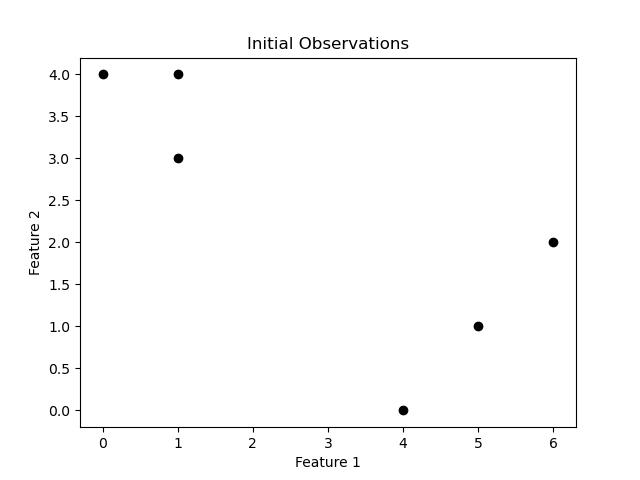
\includegraphics[width=0.8\textwidth]{images/initial_observations.jpg}
    \caption{Plot of Initial Observations}
    \label{fig:initial_observations}
\end{figure}

\newpage

\subsection{Step 2: Randomly Assign Cluster Labels}

In this step, each observation is randomly assigned to one of the two clusters, \( C_1 \) and \( C_2 \). This random assignment serves as the initial condition for the K-means algorithm.

\subsubsection*{Mathematical Context}
Let \( C_k \) represent the \( k \)-th cluster, where \( k = 1, 2 \). The initial assignment is random, meaning each data point \( \mathbf{x}_i \) is assigned a cluster label without any consideration of proximity to other points.

\subsubsection*{Code Section}

\begin{minted}[frame=lines, linenos, breaklines]{python}
# Random initial cluster assignments
cluster_labels = np.random.choice([0, 1], size=6)

# Print initial cluster assignments
print("Initial Cluster Labels:", cluster_labels)
\end{minted}

\subsubsection*{Image Section}

\begin{figure}[h!]
    \centering
    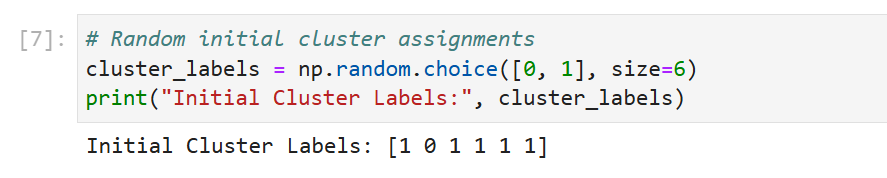
\includegraphics[width=0.6\textwidth]{images/initial_cluster_lab.png}
    \caption{Initial Random Cluster Assignments}
    \label{fig:initial_cluster_assignment}
\end{figure}

\newpage

\subsection{Step 3: Compute the Centroid for Each Cluster}

After the initial cluster assignment, the next step is to compute the centroid of each cluster. The centroid represents the center of mass of the points within the cluster.

\subsubsection*{Mathematical Formulation}
The centroid \( \mathbf{\mu}_k \) of cluster \( C_k \) is computed as:

\[
\mathbf{\mu}_k = \frac{1}{|C_k|} \sum_{\mathbf{x}_i \in C_k} \mathbf{x}_i
\]

where \( |C_k| \) is the number of points in cluster \( C_k \).

For example, if cluster \( C_1 \) consists of the points \( (1, 4), (0, 4), (6, 2) \), the centroid \( \mathbf{\mu}_1 \) is calculated as:

\[
\mathbf{\mu}_1 = \left( \frac{1+0+6}{3}, \frac{4+4+2}{3} \right) = (2.33, 3.33)
\]

\subsubsection*{Code Section}

\begin{minted}[frame=lines, linenos, breaklines]{python}
# Function to compute the centroid of each cluster
def compute_centroid(cluster_points):
    return np.mean(cluster_points, axis=0)

# Compute centroids for the initial clusters
centroids = np.array([compute_centroid(data[cluster_labels == k]) for k in range(2)])

# Print initial centroids
print("Initial Centroids:\n", centroids)
\end{minted}

\subsubsection*{Image Section}

\begin{figure}[h!]
    \centering
    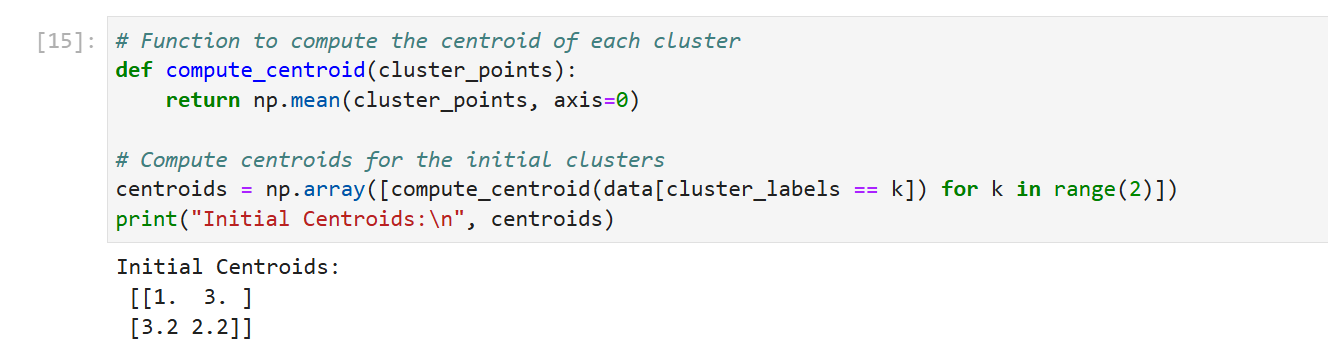
\includegraphics[width=0.8\textwidth]{images/inital_centroid.png}
    \caption{Initial Centroids of Clusters}
    \label{fig:initial_centroids}
\end{figure}

\newpage

\subsection{Step 4: Assign Each Observation to the Nearest Centroid}

After computing the centroids, each observation is reassigned to the cluster whose centroid is nearest to it, based on the Euclidean distance.

\subsubsection*{Mathematical Concept}
The Euclidean distance between a point \( \mathbf{x}_i = (x_1, y_1) \) and a centroid \( \mathbf{\mu}_k = (x_2, y_2) \) is calculated as:

\[
d(\mathbf{x}_i, \mathbf{\mu}_k) = \sqrt{(x_2 - x_1)^2 + (y_2 - y_1)^2}
\]

Each point is reassigned to the cluster \( C_k \) that minimizes this distance.

\subsubsection*{Code Section}

\begin{minted}[frame=lines, linenos, breaklines]{python}
# Reassign points to the nearest centroid
new_cluster_labels = np.array([np.argmin([np.linalg.norm(point - centroids[k]) for k in range(2)]) for point in data])

# Print new cluster assignments
print("New Cluster Labels:", new_cluster_labels)
\end{minted}

\subsubsection*{Image Section}

\begin{figure}[h!]
    \centering
    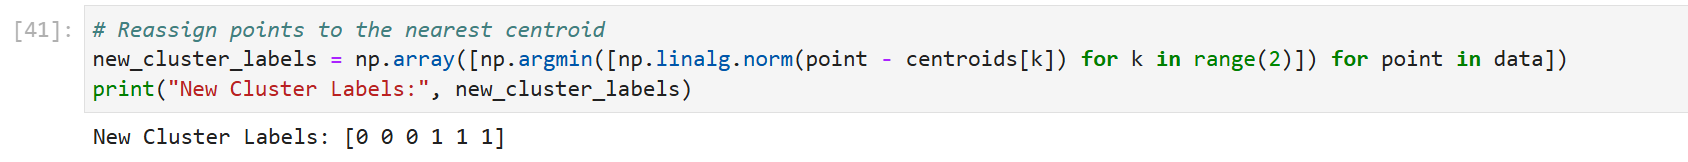
\includegraphics[width=0.8\textwidth]{images/reassigned_points.png}
    \caption{Reassigned Cluster Labels Based on Nearest Centroid}
    \label{fig:reassigned_clusters}
\end{figure}

\newpage

\subsection{Step 5: Repeat Until Convergence}

The steps of recalculating centroids and reassigning points are repeated iteratively until the cluster assignments stabilize, meaning they no longer change. This point of stabilization is referred to as convergence.

\subsubsection*{Mathematical Criterion for Convergence}
Convergence is achieved when the centroids no longer move, and the cluster assignments of the data points do not change between iterations. Mathematically, this can be expressed as:

\[
\mathbf{c}^{(t+1)} = \mathbf{c}^{(t)}
\]

where \( \mathbf{c}^{(t)} \) denotes the centroid vector at the \( t \)-th iteration.

\subsubsection*{Code Section}

\begin{minted}[frame=lines, linenos, breaklines]{python}
# Iterative K-means steps until convergence
for iteration in range(10):  # Limit iterations to avoid infinite loops
    centroids = np.array([compute_centroid(data[cluster_labels == k]) for k in range(2)])
    new_cluster_labels = np.array([np.argmin([np.linalg.norm(point - centroids[k]) for k in range(2)]) for point in data])
    
    if np.array_equal(new_cluster_labels, cluster_labels):
        break  # Convergence reached
    
    cluster_labels = new_cluster_labels

# Final cluster labels and centroids after convergence
print("Final Cluster Labels:", cluster_labels)
print("Final Centroids:\n", centroids)
\end{minted}

\subsubsection*{Image Section}

\begin{figure}[h!]
    \centering
    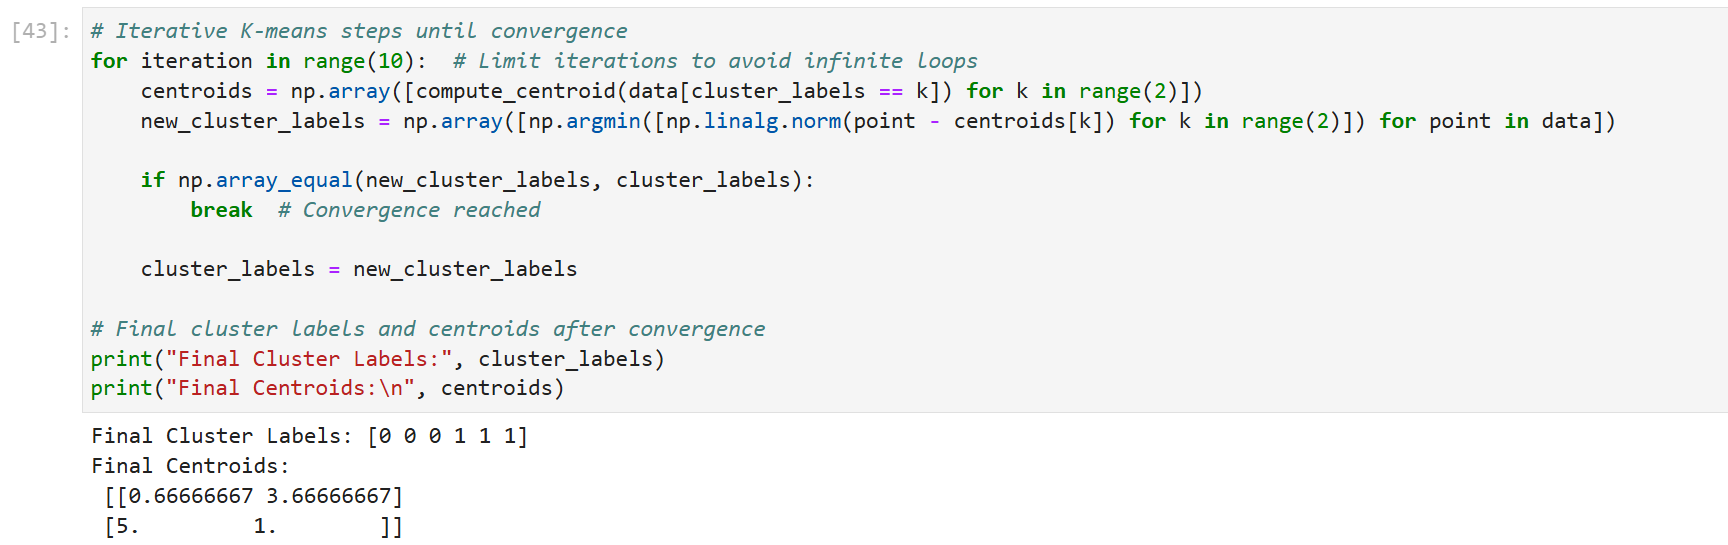
\includegraphics[width=0.8\textwidth]{images/final_cluster_value.png}
    \caption{Final Cluster Assignments After Convergence}
    \label{fig:final_clusters}
\end{figure}

\newpage

\subsection{Step 6: Visualize Final Clusters}

In the final step, we visualize the clusters by coloring the observations according to their final cluster labels.

\subsubsection*{Code Section}

\begin{minted}[frame=lines, linenos, breaklines]{python}
# Plot final clusters
plt.subplot(1, 2, 1)  # 2D plot of the final clusters
plt.scatter(data[:, 0], data[:, 1], c=cluster_labels)
plt.scatter(centroids[:, 0], centroids[:, 1], c='red', marker='x')
plt.title('Final Cluster Assignments (2D)')
plt.xlabel('Feature 1')
plt.ylabel('Feature 2')

plt.subplot(1, 2, 2)  # 1D plot of the final clusters (projected onto x-axis)
plt.scatter(data[:, 0], np.zeros_like(data[:, 0]), c=cluster_labels)
plt.scatter(centroids[:, 0], np.zeros_like(centroids[:, 0]), c='red', marker='x')
plt.title('Final Cluster Assignments (1D)')
plt.xlabel('Feature 1')

plt.tight_layout()
plt.savefig('./images/final_clusters_2D_1D.jpg')  # Save the combined 2D and 1D clusters as a JPG file
plt.show()
\end{minted}

\subsubsection*{Image Section}

\begin{figure}[h!]
    \centering
    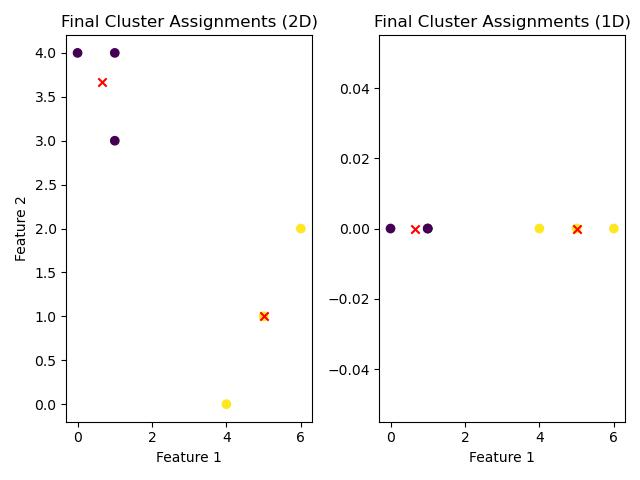
\includegraphics[width=0.6\textwidth]{images/final_clusters_2D_1D.jpg}
    \caption{Final Cluster Visualization}
    \label{fig:final_cluster_visualization}
\end{figure}


\newpage

K-means clustering is an iterative and unsupervised learning algorithm designed to partition a dataset into \( K \) distinct clusters. Through repeated reassignment and centroid recalculation, the algorithm minimizes the within-cluster variance. The K-means clustering process has successfully grouped the observations into two clusters. The centroids calculated, and the final cluster assignments remained consistent after one iteration, indicating convergence.


\section{Question 03}

\begin{quote}
Consider a 2-D data set having two types of data point class, namely X1 and X2. Given, \( X1 = (x_1, x_2) = (4, 1), (2, 4), (2, 3), (3, 6), (4, 4) \) and \( X2 = (x_1, x_2) = (9, 10), (6, 8), (9, 5), (8, 7), (10, 8) \).
\begin{itemize}
\item[(a)] Apply Linear Discriminant Analysis in the view of dimensionality reduction.
\item[(b)] Plot the graphs if required.
\item[(c)] Write advantages, disadvantages, and applications of Linear Discriminant Analysis (LDA).
\end{itemize}
\end{quote}

\subsection{Answer:}

\textbf{Given:}

We have two sets of 2D data points corresponding to two different classes \( X1 \) and \( X2 \):

\[
X1 = \begin{pmatrix} 4 & 1 \\ 2 & 4 \\ 2 & 3 \\ 3 & 6 \\ 4 & 4 \end{pmatrix}, \quad X2 = \begin{pmatrix} 9 & 10 \\ 6 & 8 \\ 9 & 5 \\ 8 & 7 \\ 10 & 8 \end{pmatrix}
\]

\textbf{To Find:} 
\begin{itemize}
    \item Apply Linear Discriminant Analysis (LDA) for dimensionality reduction.
    \item Plot the results, if necessary.
    \item Discuss the advantages, disadvantages, and applications of LDA.
\end{itemize}

\textbf{Solution:}

\subsection{Step 1: Compute the Mean Vectors}

The first step in LDA is to compute the mean vector for each class. The mean vector represents the average position of the data points within each class in the feature space.

\subsubsection*{Mathematical Formulation}

The mean vector \( \mathbf{\mu}_k \) for class \( X_k \) is calculated as:

\[
\mathbf{\mu}_k = \frac{1}{|X_k|} \sum_{\mathbf{x}_i \in X_k} \mathbf{x}_i
\]

For example, the mean vector for class \( X_1 \) is:

\[
\mathbf{\mu}_1 = \frac{1}{5} \left( (4,1) + (2,4) + (2,3) + (3,6) + (4,4) \right) = (3, 3.6)
\]

Similarly, for class \( X_2 \):

\[
\mathbf{\mu}_2 = \frac{1}{5} \left( (9,10) + (6,8) + (9,5) + (8,7) + (10,8) \right) = (8.4, 7.6)
\]

\subsubsection*{Code Section}

\begin{minted}[frame=lines, linenos, breaklines]{python}
import numpy as np

# Define the dataset
X1 = np.array([[4, 1], [2, 4], [2, 3], [3, 6], [4, 4]])
X2 = np.array([[9, 10], [6, 8], [9, 5], [8, 7], [10, 8]])

# Compute the means of each class
mean_X1 = np.mean(X1, axis=0)
mean_X2 = np.mean(X2, axis=0)

print("Mean of X1:", mean_X1)
print("Mean of X2:", mean_X2)
\end{minted}

\subsubsection*{Image Section}

\begin{figure}[h!]
    \centering
    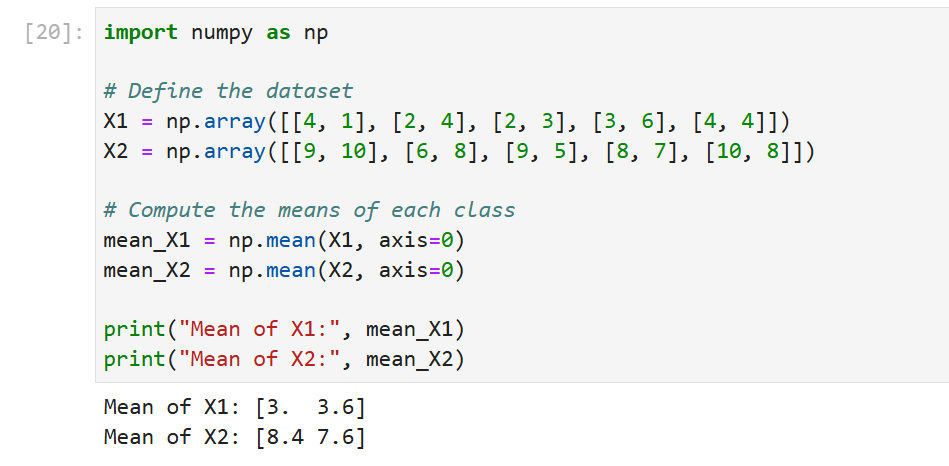
\includegraphics[width=0.8\textwidth]{images/mean_x1_x2.png}
    \caption{Computed Mean Vectors for X1 and X2}
    \label{fig:mean_x1_x2}
\end{figure}

\newpage

\subsection{Step 2: Compute the Scatter Matrices}

LDA involves computing the within-class scatter matrix \( S_W \) and the between-class scatter matrix \( S_B \). These matrices capture the variance within each class and the variance between the classes, respectively.

\subsubsection*{Mathematical Formulation}

The within-class scatter matrix \( S_W \) is given by:

\[
S_W = \sum_{k=1}^{2} \sum_{\mathbf{x}_i \in X_k} (\mathbf{x}_i - \mathbf{\mu}_k)(\mathbf{x}_i - \mathbf{\mu}_k)^\top
\]

The between-class scatter matrix \( S_B \) is defined as:

\[
S_B = \sum_{k=1}^{2} N_k (\mathbf{\mu}_k - \mathbf{\mu})(\mathbf{\mu}_k - \mathbf{\mu})^\top
\]

where \( \mathbf{\mu} \) is the overall mean vector:

\[
\mathbf{\mu} = \frac{N_1 \mathbf{\mu}_1 + N_2 \mathbf{\mu}_2}{N_1 + N_2}
\]

\subsubsection*{Code Section}

\begin{minted}[frame=lines, linenos, breaklines]{python}
# Compute the within-class scatter matrix
S_W = np.zeros((2, 2))
for x in X1:
    S_W += np.dot((x - mean_X1).reshape(2, 1), (x - mean_X1).reshape(1, 2))
for x in X2:
    S_W += np.dot((x - mean_X2).reshape(2, 1), (x - mean_X2).reshape(1, 2))

# Compute the between-class scatter matrix
mean_overall = np.mean(np.vstack((X1, X2)), axis=0)
S_B = np.dot((mean_X1 - mean_overall).reshape(2, 1), (mean_X1 - mean_overall).reshape(1, 2)) * X1.shape[0] + \
      np.dot((mean_X2 - mean_overall).reshape(2, 1), (mean_X2 - mean_overall).reshape(1, 2)) * X2.shape[0]

print("Within-class Scatter Matrix SW:\n", S_W)
print("Between-class Scatter Matrix SB:\n", S_B)
\end{minted}

\subsubsection*{Image Section}

\begin{figure}[h!]
    \centering
    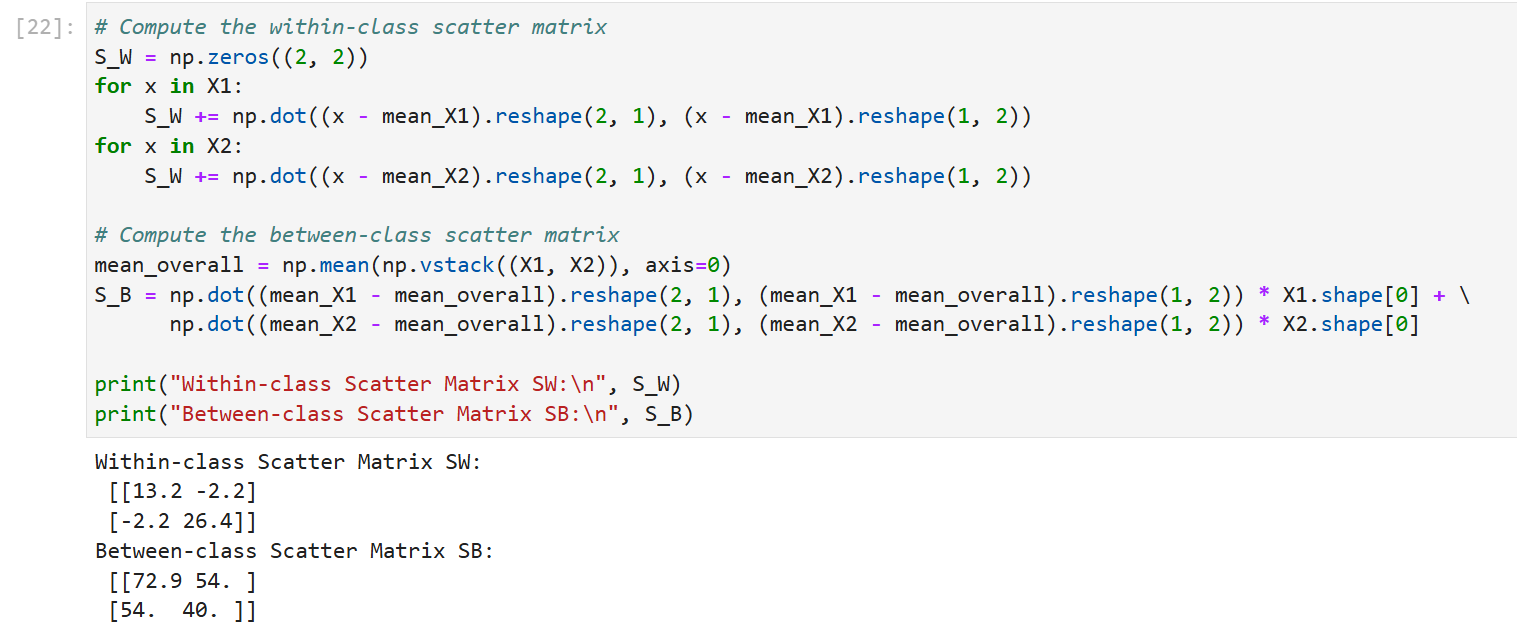
\includegraphics[width=0.8\textwidth]{images/scatter_matrices.png}
    \caption{Within-class and Between-class Scatter Matrices}
    \label{fig:scatter_matrices}
\end{figure}

\newpage

\subsection{Step 3: Compute the LDA Projection}

The next step involves finding the linear discriminant that maximizes the ratio of the between-class scatter to the within-class scatter. This discriminant is the direction that best separates the two classes.

\subsubsection*{Mathematical Formulation}

The linear discriminant \( \mathbf{w} \) is obtained by solving the following eigenvalue problem:

\[
S_W^{-1} S_B \mathbf{w} = \lambda \mathbf{w}
\]

We choose the eigenvector \( \mathbf{w} \) corresponding to the largest eigenvalue \( \lambda \).

\subsubsection*{Code Section}

\begin{minted}[frame=lines, linenos, breaklines]{python}
# Solve the eigenvalue problem for the matrix SW^-1 * SB
eig_vals, eig_vecs = np.linalg.eig(np.linalg.inv(S_W).dot(S_B))

# Select the eigenvector with the largest eigenvalue
w = eig_vecs[:, np.argmax(eig_vals)]

print("Linear Discriminant Vector w:", w)
\end{minted}

\subsubsection*{Image Section}

\begin{figure}[h!]
    \centering
    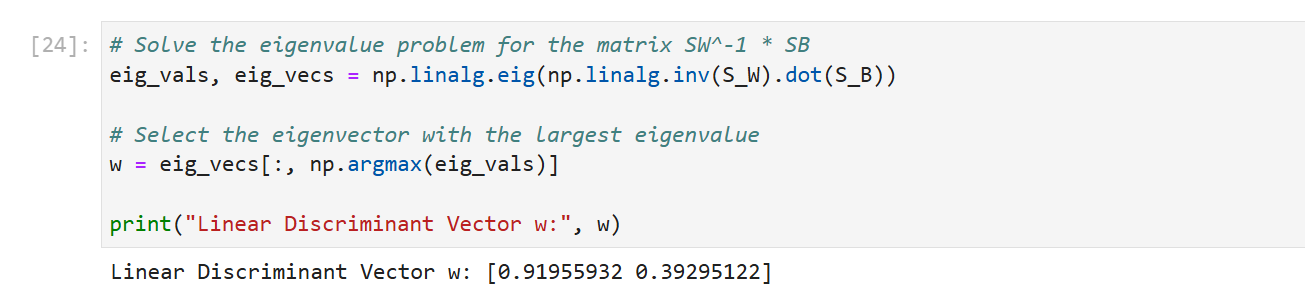
\includegraphics[width=0.8\textwidth]{images/lda_vector.png}
    \caption{Linear Discriminant Vector \( \mathbf{w} \)}
    \label{fig:lda_vector}
\end{figure}

\newpage

\subsection{Step 4: Project the Data onto the Linear Discriminant}

Once the linear discriminant vector \( \mathbf{w} \) is identified, the data points are projected onto this vector to achieve dimensionality reduction.

\subsubsection*{Mathematical Concept}

The projection of a data point \( \mathbf{x} \) onto the linear discriminant \( \mathbf{w} \) is computed as:

\[
y = \mathbf{w}^\top \mathbf{x}
\]

This projection reduces the dimensionality from 2D to 1D along the direction that maximizes the separation between the two classes.

\subsubsection*{Code Section}

\begin{minted}[frame=lines, linenos, breaklines]{python}
# Project the data onto the linear discriminant
X1_proj = X1.dot(w)
X2_proj = X2.dot(w)

print("Projected Data X1:", X1_proj)
print("Projected Data X2:", X2_proj)
\end{minted}

\subsubsection*{Image Section}

\begin{figure}[h!]
    \centering
    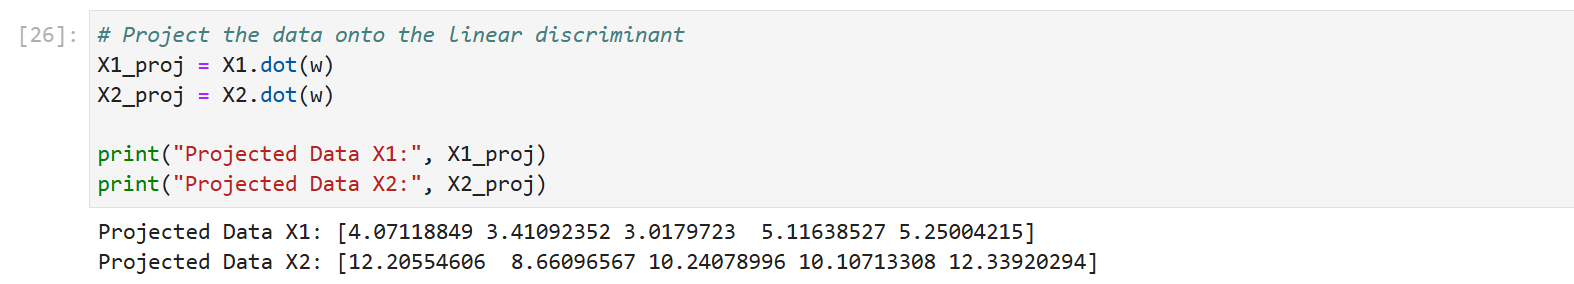
\includegraphics[width=0.8\textwidth]{images/lda_projection.png}
    \caption{Projection of Data onto Linear Discriminant}
    \label{fig:lda_projection}
\end{figure}

\newpage

\subsection{Step 5: Discuss the Advantages, Disadvantages, and Applications of LDA}

\textbf{Advantages:}
\begin{itemize}
    \item LDA maximizes class separability by projecting data onto a lower-dimensional space, making it particularly effective for classification tasks.
    \item It works well with linearly separable data, providing clear decision boundaries between classes.
    \item LDA is computationally efficient and straightforward to implement, making it suitable for high-dimensional datasets.
\end{itemize}

\textbf{Disadvantages:}
\begin{itemize}
    \item LDA assumes that classes have identical covariance matrices, which may not always hold true in real-world datasets.
    \item It is not effective for non-linearly separable data, as it can only create linear decision boundaries.
    \item LDA can be sensitive to outliers, which can significantly affect the calculated discriminant.
\end{itemize}

\textbf{Applications:}
\begin{itemize}
    \item LDA is widely used in pattern recognition and face recognition, where distinguishing between different classes is crucial.
    \item It is also used for dimensionality reduction before applying other machine learning algorithms, helping to improve performance and reduce computational complexity.
    \item LDA is applied in various classification tasks, especially when the number of features is large compared to the number of samples, such as in text classification and bioinformatics.
\end{itemize}


\section{Question 04}

\begin{quote}
For the \textbf{Wine Quality Data Set}, convert all the values in the quality attribute to 0 (bad) if the value is less than or equal to 6 and to 1 (good) otherwise. Normalize all the other attributes between 0 and 1 by min-max scaling. Mention why we use min-max scaling.
\end{quote}

\subsection{Answer:}

\textbf{Given:}

We are required to work with the Wine Quality Data Set, where the goal is to convert the quality attribute values and normalize the other attributes using min-max scaling.

\textbf{To Find:} 
\begin{itemize}
    \item Convert the quality attribute values based on the condition given.
    \item Normalize the remaining features using min-max scaling.
\end{itemize}

\textbf{Solution:}

\subsubsection{Step 1: Load the Wine Dataset}

We begin by loading the wine dataset using pandas:

\begin{minted}[frame=lines, linenos, breaklines]{python}
import pandas as pd

# Load the dataset from the CSV file
df = pd.read_csv('./dataset/WineQT.csv')

# Display the first few rows of the dataset
print(df.head())
\end{minted}

The dataset consists of multiple attributes related to wine characteristics, and a target attribute representing the wine quality class.

\subsubsection*{Image Section}

\begin{figure}[h!]
    \centering
    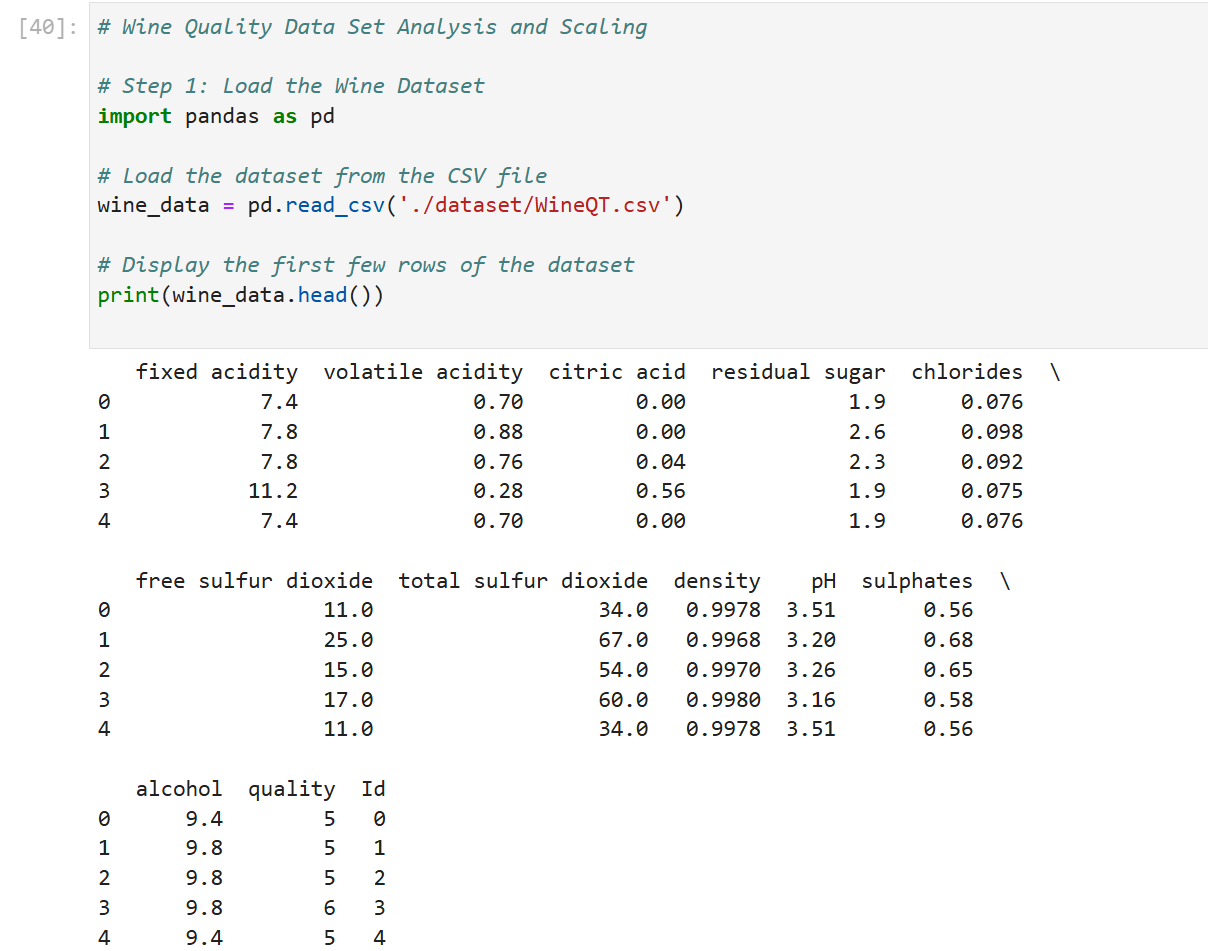
\includegraphics[width=0.8\textwidth]{images/wine_dataset_head.png}
    \caption{First Five Rows of Wine Quality Dataset}
    \label{fig:wine_dataset_head}
\end{figure}

\newpage

\subsubsection{Step 2: Convert the Quality Attribute}

Next, we convert the quality attribute values to 0 (bad) if the value is less than or equal to 6 and to 1 (good) otherwise.

\begin{minted}[frame=lines, linenos, breaklines]{python}
# Convert quality attribute
df['quality'] = df['quality'].apply(lambda x: 0 if x <= 6 else 1)

# Display the first few rows after conversion
print(df[['quality']].head())
\end{minted}

This code converts the wine quality based on the conditions provided.

\subsubsection*{Image Section}

\begin{figure}[h!]
    \centering
    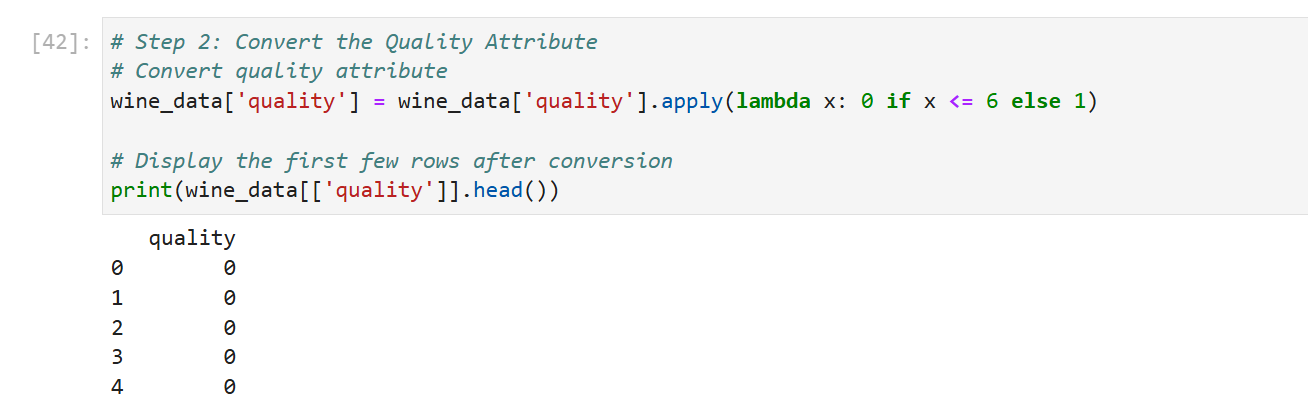
\includegraphics[width=0.8\textwidth]{images/quality_conversion.png}
    \caption{Quality Attribute After Conversion}
    \label{fig:quality_conversion}
\end{figure}

\newpage

\subsubsection{Step 3: Normalize the Attributes using Min-Max Scaling}

We normalize the other attributes between 0 and 1 using min-max scaling. Min-max scaling transforms features to a fixed range [0, 1].

\[
\text{Min-Max Scaling Formula: } x' = \frac{x - \min(x)}{\max(x) - \min(x)}
\]

\begin{minted}[frame=lines, linenos, breaklines]{python}
from sklearn.preprocessing import MinMaxScaler

# Initialize the MinMaxScaler
scaler = MinMaxScaler()

# Scale all features except for 'quality'
scaled_features = scaler.fit_transform(wine_data.drop(columns=['quality']))

# Convert the scaled features back to a DataFrame
df_scaled = pd.DataFrame(scaled_features, columns=wine_data.columns[:-1])

# Add the 'quality' column back to the scaled DataFrame
df_scaled['quality'] = wine_data['quality']

# Display the first few rows of the scaled dataset
print(df_scaled.head())
\end{minted}

This code uses `MinMaxScaler` from `sklearn.preprocessing` to scale the data.

\subsubsection*{Image Section}

\begin{figure}[h!]
    \centering
    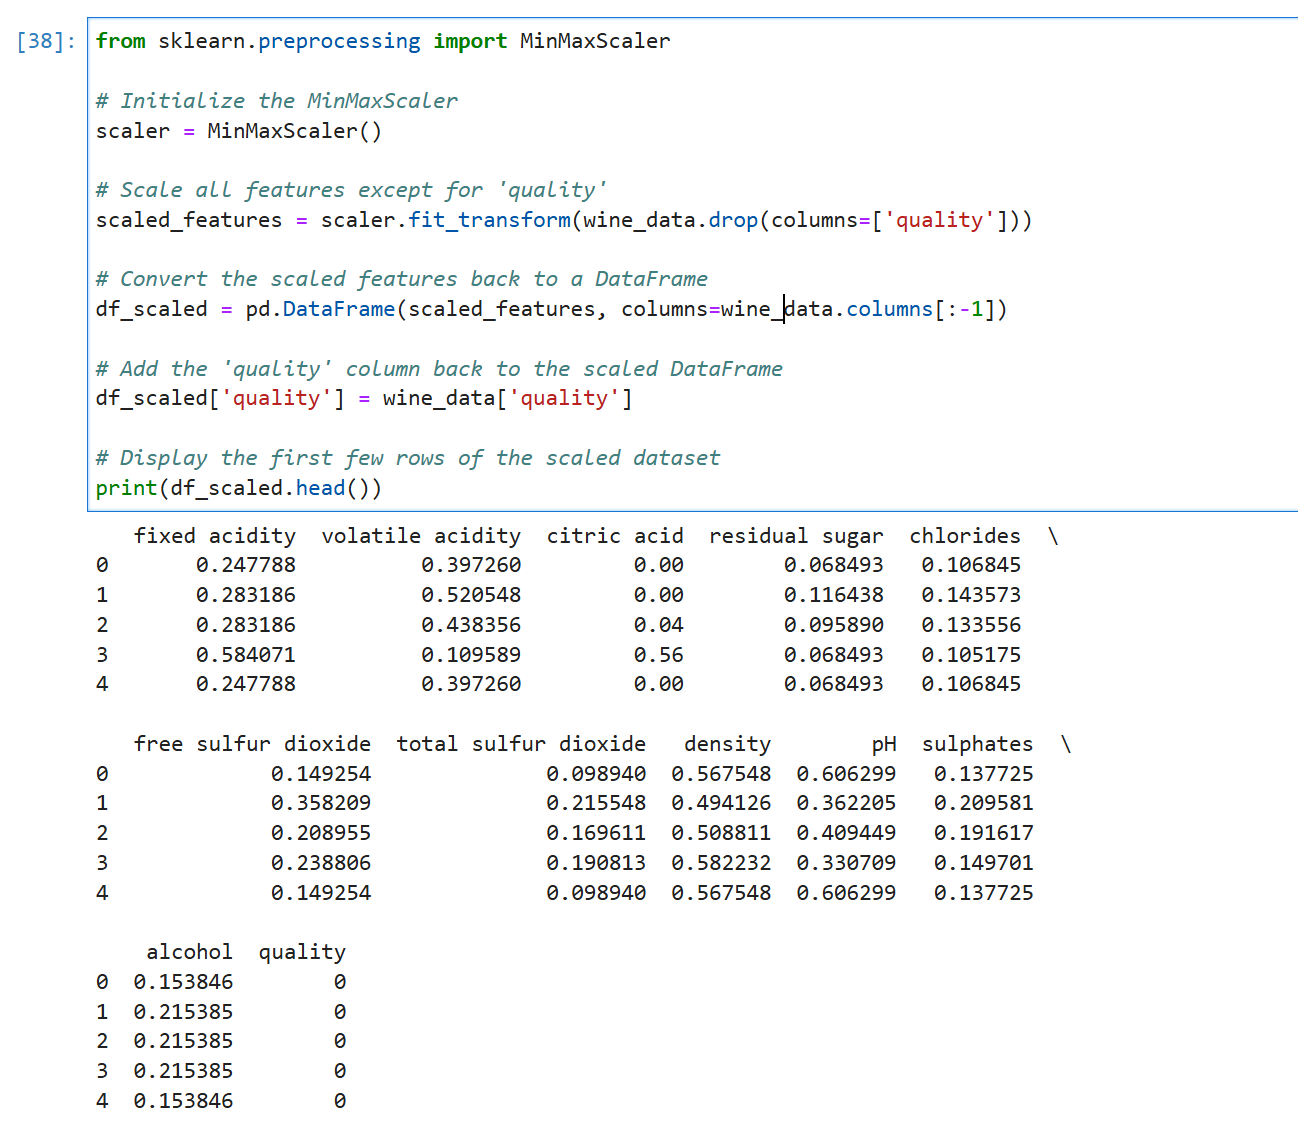
\includegraphics[width=0.8\textwidth]{images/wine_scaled_data.png}
    \caption{Scaled Features and Quality Attribute}
    \label{fig:step_3_scaled_data}
\end{figure}

\newpage

\subsubsection{Step 4: Plot the Data Before and After Scaling}

To visualize the effect of min-max scaling, we plot the data before and after scaling:

\begin{minted}[frame=lines, linenos, breaklines]{python}
import matplotlib.pyplot as plt

# Plotting before scaling
plt.figure(figsize=(14, 8))

# Plotting the data before scaling
plt.subplot(1, 2, 1)
plt.boxplot(df.drop(columns=['quality']).values)
plt.title('Before Scaling')
plt.xticks(range(1, len(df.columns)), df.columns.drop('quality'), rotation=90)

# Plotting after scaling
plt.subplot(1, 2, 2)
plt.boxplot(df_scaled.drop(columns=['quality']).values)
plt.title('After Min-Max Scaling')
plt.xticks(range(1, len(df_scaled.columns)), df_scaled.columns.drop('quality'), rotation=90)

plt.tight_layout()
plt.show()
\end{minted}

\begin{figure}[h!]
    \centering
    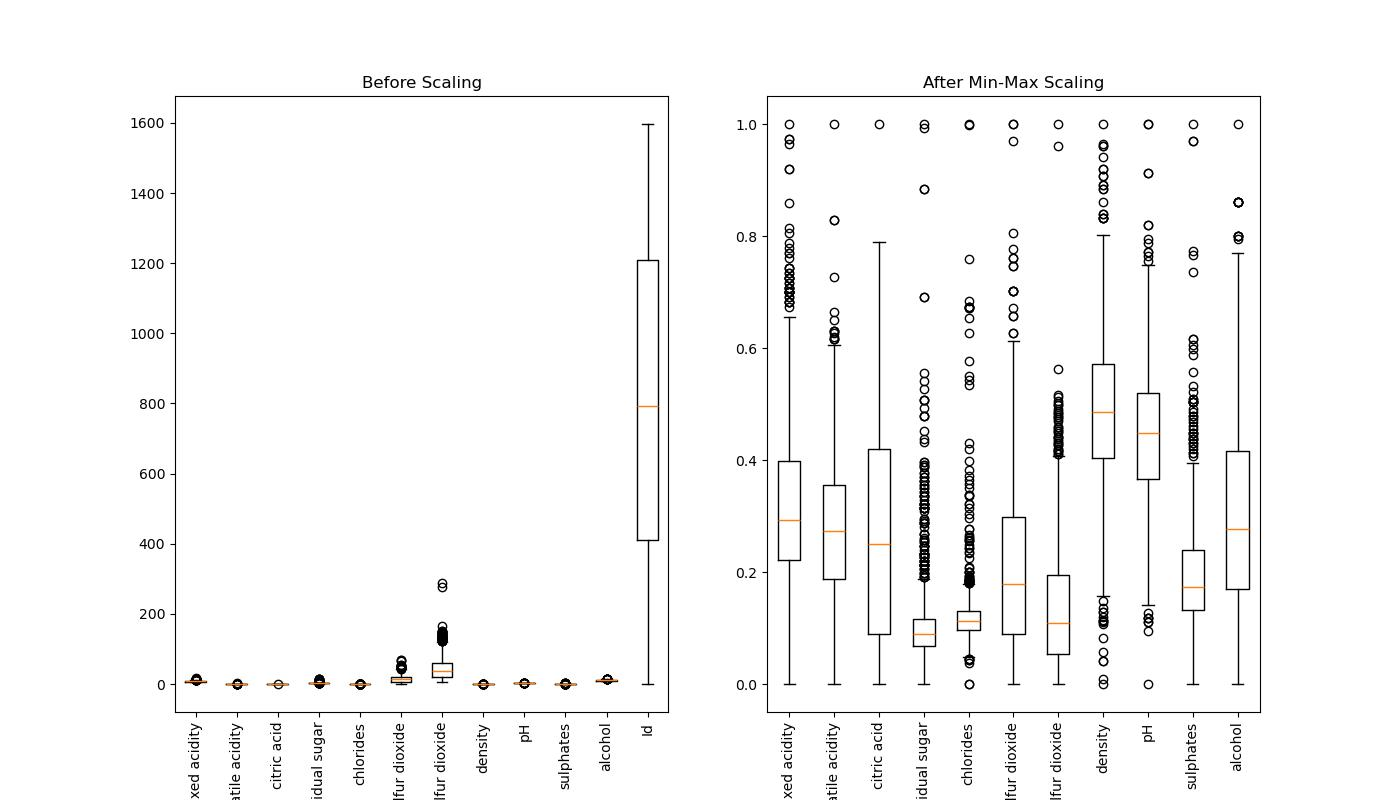
\includegraphics[width=0.9\textwidth]{images/scaling_comparison_plot.jpg}
    \caption{Comparison of Data Distribution Before and After Scaling}
    \label{fig:scaling_comparison}
\end{figure}

These boxplots show the distribution of the data before and after scaling. After min-max scaling, all features are in the range [0, 1].

\subsubsection{Step 5: Explain Why We Use Min-Max Scaling}

\textbf{Why Use Min-Max Scaling?}
\begin{itemize}
    \item Min-max scaling is essential when features have different units or scales, which can bias the model's performance.
    \item It ensures that all features contribute equally to the distance calculations in algorithms such as K-means clustering or nearest neighbors.
    \item Min-max scaling is particularly useful when the model is sensitive to the magnitude of features, such as in gradient descent optimization.
\end{itemize}

\textbf{Result:} The quality attribute has been successfully converted, and the remaining features have been normalized using min-max scaling.

\subsubsection{GitHub Link}

Please refer to the following GitHub repository for the complete code and output in the \texttt{.ipynb} file:

\href{https://github.com/Nitin-Mane/CS550-Machine-Learning-Assignment/tree/main/Assignment_03}{GitHub Link}

\textbf{Note:} Please check the Notebook filename: \texttt{NitinMane\_M24MT004\_Assignment01.ipynb}

\section{Question 05}

\begin{quote}
What is the difference between model parameters and model hyperparameters? What is meant by hyperparameter tuning? Name some common hyperparameters used in clustering algorithms.
\end{quote}

\subsection{Answer:}

\subsubsection{Model Parameters vs. Hyperparameters}

The following table highlights the key differences between model parameters and model hyperparameters:

\begin{center}
\begin{tabular}{|p{7cm}|p{7cm}|}
\hline
\textbf{Model Parameters} & \textbf{Model Hyperparameters} \\
\hline
Learned from the data during the training process. & Set before the training process begins. \\
\hline
Examples include weights in a neural network, coefficients in linear regression. & Examples include learning rate, number of layers in a neural network, number of clusters in K-means. \\
\hline
Influence the predictions made by the model. & Influence how the model is trained or the model structure itself. \\
\hline
Optimized by algorithms such as gradient descent. & Optimized through methods like grid search, random search, or Bayesian optimization. \\
\hline
Typically have values that can be adjusted continuously. & Often require discrete values or categorical choices. \\
\hline
Directly impact the model's accuracy and performance. & Impact the model's training time, complexity, and generalization ability. \\
\hline
\end{tabular}
\end{center}

\subsubsection{Hyperparameter Tuning}

\textbf{Definition:}

Hyperparameter tuning is the process of finding the optimal set of hyperparameters for a machine learning model. Unlike model parameters, which are learned during the training process, hyperparameters are set before the training process begins. The goal of hyperparameter tuning is to improve the model's performance by selecting the best possible values for these hyperparameters.

\textbf{Methods for Hyperparameter Tuning:}
\begin{itemize}
    \item \textbf{Grid Search:} A systematic approach where all possible combinations of hyperparameters are tried, and the best one is selected based on model performance.
    \item \textbf{Random Search:} A more efficient approach where random combinations of hyperparameters are tested, and the best one is selected.
    \item \textbf{Bayesian Optimization:} A probabilistic model-based approach that aims to find the best hyperparameters more efficiently by modeling the performance as a function of the hyperparameters.
\end{itemize}

\subsubsection{Prevalent Hyperparameters in Clustering Algorithms}

In the domain of clustering algorithms, several hyperparameters are instrumental in determining the performance and outcomes of these methods:

\begin{itemize} 
 \item \textbf{Number of Clusters (K):} This hyperparameter specifies the predetermined number of clusters that the algorithm, such as K-means, is required to partition the data into.
 \item \textbf{Distance Metric:} This parameter delineates the metric employed to measure distances between data points, encompassing methods such as Euclidean distance or Manhattan distance.
 \item \textbf{Initialization Method:} The strategy utilized for initializing the centroids in K-means, with options including 'random' or 'k-means++'.
 \item \textbf{Maximum Iterations:} This defines the upper bound on the number of iterations the algorithm will execute prior to termination.
 \item \textbf{Convergence Tolerance:} The specified threshold at which the algorithm ceases execution if the alterations in centroids fall below this value.
 \item \textbf{Linkage Criterion (in Hierarchical Clustering):} The criterion governing the amalgamation of clusters, examples of which include 'single', 'complete', or 'average' linkage.
\end{itemize}

\section{Question 06}

\begin{quote}
You are given three observed signals \( x_1(t) \), \( x_2(t) \), and \( x_3(t) \) which are linear mixtures of three independent source signals \( s_1(t) \), \( s_2(t) \), and \( s_3(t) \). The mixing process is represented by the following matrix equation:

\[
\mathbf{x}(t) = \mathbf{A} \mathbf{s}(t)
\]

where

\[
\mathbf{x}(t) = \begin{pmatrix} x_1(t) \\ x_2(t) \\ x_3(t) \end{pmatrix}, \quad \mathbf{s}(t) = \begin{pmatrix} s_1(t) \\ s_2(t) \\ s_3(t) \end{pmatrix}, \quad \mathbf{A} = \begin{pmatrix} a_{11} & a_{12} & a_{13} \\ a_{21} & a_{22} & a_{23} \\ a_{31} & a_{32} & a_{33} \end{pmatrix}
\]

where \( \mathbf{A} \) is an unknown \( 3 \times 3 \) mixing matrix, and \( \mathbf{s}(t) \) represents the independent source signals.
\end{quote}

\subsection{(a) Explain the steps involved in estimating the mixing matrix \texorpdfstring{$\mathbf{A}$}{A} and the independent source signals \texorpdfstring{$\mathbf{s}(t)$}{s(t)} using ICA.}

\textbf{Answer:}

\subsubsection{Introduction to ICA}

Independent Component Analysis (ICA) is a computational technique used to separate a multivariate signal into additive independent components. It is based on the assumption that the observed signals are linear mixtures of independent source signals. The objective is to estimate both the mixing matrix \( \mathbf{A} \) and the original source signals \( \mathbf{s}(t) \) from the observed signals \( \mathbf{x}(t) \).

\subsubsection{Step 1: Centering the Data}

Centering the data is the first step in ICA, which involves subtracting the mean from each observed signal to ensure that the data has a zero mean. This simplifies subsequent calculations:

\[
\mathbf{x}_{\text{centered}}(t) = \mathbf{x}(t) - \mathbb{E}[\mathbf{x}(t)]
\]

Here, \( \mathbb{E}[\mathbf{x}(t)] \) is the mean of the observed signals over time.

\subsubsection{Step 2: Whitening the Data}

Whitening transforms the centered data so that the components are uncorrelated and have unit variance. Whitening is done by calculating the covariance matrix of the centered data:

\[
\mathbf{C}_{\mathbf{x}} = \mathbb{E}[\mathbf{x}_{\text{centered}}(t) \mathbf{x}_{\text{centered}}^\top(t)]
\]

Next, we perform an eigenvalue decomposition of the covariance matrix:

\[
\mathbf{C}_{\mathbf{x}} = \mathbf{E} \mathbf{D} \mathbf{E}^\top
\]

where \( \mathbf{E} \) is the matrix of eigenvectors, and \( \mathbf{D} \) is the diagonal matrix of eigenvalues. The whitening transformation is then applied:

\[
\mathbf{z}(t) = \mathbf{D}^{-1/2} \mathbf{E}^\top \mathbf{x}_{\text{centered}}(t)
\]

This transformation ensures that \( \mathbf{z}(t) \) is uncorrelated with unit variance.

\subsubsection{Step 3: Estimating the Mixing Matrix \texorpdfstring{$\mathbf{A}$}{A}}

The key goal of ICA is to estimate the mixing matrix \( \mathbf{A} \). This is done by finding a matrix \( \mathbf{W} \) such that the components of \( \mathbf{W} \mathbf{z}(t) \) are as independent as possible. The FastICA algorithm is a commonly used method, which involves the following steps:

\begin{enumerate}
    \item\textbf{Choose an initial guess} for the matrix \( \mathbf{W} \).
    \item \textbf{Iteratively update} \( \mathbf{W} \) using the following rule:
    \[
    \mathbf{w}_{\text{new}} = \mathbb{E}[\mathbf{z}(t) g(\mathbf{w}^\top \mathbf{z}(t))] - \mathbb{E}[g'(\mathbf{w}^\top \mathbf{z}(t))] \mathbf{w}
    \]
    where \( g(\cdot) \) is a non-linear function (e.g., \( g(u) = \tanh(u) \)), and \( g'(u) \) is its derivative.
    \item \textbf{Normalize} \( \mathbf{w}_{\text{new}} \) to have unit norm.
    \item \textbf{Check for convergence}: If the change in \( \mathbf{W} \) is below a threshold, the algorithm has converged.
\end{enumerate}

The resulting matrix \( \mathbf{W} \) is the estimated unmixing matrix, and its inverse gives the estimated mixing matrix:

\[
\mathbf{A} \approx \mathbf{W}^{-1}
\]

\subsubsection{Step 4: Recovering the Source Signals \texorpdfstring{$\mathbf{s}(t)$}{s(t)}}

Once the unmixing matrix \( \mathbf{W} \) is estimated, the independent source signals \( \mathbf{s}(t) \) can be recovered by:

\[
\mathbf{s}(t) = \mathbf{W} \mathbf{z}(t)
\]

Since \( \mathbf{z}(t) = \mathbf{D}^{-1/2} \mathbf{E}^\top \mathbf{x}_{\text{centered}}(t) \), the source signals can be expressed as:

\[
\mathbf{s}(t) = \mathbf{W} \mathbf{D}^{-1/2} \mathbf{E}^\top \left(\mathbf{x}(t) - \mathbb{E}[\mathbf{x}(t)]\right)
\]

Thus, \( \mathbf{s}(t) \) is recovered by applying the estimated unmixing matrix to the whitened, centered data.

The process of ICA involves centering and whitening the observed data, estimating the mixing matrix using FastICA, and recovering the independent source signals. This process hinges on the statistical independence and non-Gaussianity of the source signals.

\subsection{(b) Suppose the mixing matrix \texorpdfstring{$\mathbf{A}$}{A} is not full rank (i.e., it is singular or nearly singular). How would this affect the ICA process? Discuss the potential challenges and the implications for recovering the original source signals.}

\textbf{Answer:}

\subsubsection{Implications of a Non-Full Rank Mixing Matrix}

A non-full rank mixing matrix \( \mathbf{A} \) significantly complicates the ICA process. Here’s why:

\begin{itemize}
    \item \textbf{Underdetermined System:} A non-full rank matrix \( \mathbf{A} \) implies that the system \( \mathbf{x}(t) = \mathbf{A} \mathbf{s}(t) \) is underdetermined, meaning there are more unknowns (source signals) than equations (observed signals). This makes it impossible to uniquely solve for the source signals \( \mathbf{s}(t) \).
    
    \item \textbf{Loss of Information:} A singular matrix \( \mathbf{A} \) indicates that some of the original source information has been lost during the mixing process, making it impossible to fully recover the original signals. This loss of information typically occurs when distinct source signals are projected onto the same or nearly the same direction in the observed space.
    
    \item \textbf{Inversion Issues:} The ICA process requires the inversion of the mixing matrix \( \mathbf{A} \) to recover the source signals. If \( \mathbf{A} \) is singular or nearly singular, it cannot be inverted, which prevents the direct recovery of the source signals.
    
    \item \textbf{Dependence Among Sources:} A non-full rank \( \mathbf{A} \) suggests that the source signals are not truly independent, violating one of the core assumptions of ICA. Without independence, the algorithm cannot effectively separate the mixed signals.
\end{itemize}

\subsubsection{Challenges and Practical Implications}

\begin{itemize}
    \item \textbf{Algorithmic Instability:} Near-singular matrices can lead to numerical instability during the inversion process, causing the algorithm to produce inaccurate or completely erroneous results.
    
    \item \textbf{Limited Signal Separation:} When \( \mathbf{A} \) is not full rank, the separation of signals is compromised. The ICA algorithm may fail to separate the signals entirely, resulting in outputs that are mixtures or combinations of the original source signals.
    
    \item \textbf{Preprocessing with PCA:} In cases where the mixing matrix is nearly singular, preprocessing with techniques like Principal Component Analysis (PCA) can help reduce the dimensionality and mitigate some of the challenges, although it may not completely resolve the issue.
    
    \item \textbf{Increased Computational Complexity:} Dealing with a non-full rank matrix often requires additional computational steps, such as regularization or dimensionality reduction, which increases the overall complexity of the ICA process.
\end{itemize}

The success of ICA relies heavily on the assumption that the mixing matrix \( \mathbf{A} \) is full-rank and invertible. If this condition is not met, the separation of the independent source signals becomes highly challenging, if not impossible. In such cases, additional preprocessing steps or alternative methods may be required to achieve any meaningful separation of the signals.


\textbf{Answer:}

\subsubsection{Introduction to ICA}

Independent Component Analysis (ICA) is a computational technique used to separate a multivariate signal into additive, independent components. The central task is to estimate both the mixing matrix \( \mathbf{A} \) and the source signals \( \mathbf{s}(t) \) from the observed signals \( \mathbf{x}(t) \).

Given the linear relationship:
\[
\mathbf{x}(t) = \mathbf{A} \mathbf{s}(t)
\]
where \( \mathbf{A} \) is an unknown mixing matrix, the goal of ICA is to recover \( \mathbf{s}(t) \) and estimate \( \mathbf{A} \) under the assumption that the components of \( \mathbf{s}(t) \) are statistically independent.

\subsubsection{Step 1: Centering the Data}

The first step in ICA is to center the observed data \( \mathbf{x}(t) \). Centering involves subtracting the mean of the data to ensure that it has a zero mean. This can be mathematically expressed as:

\[
\mathbf{x}_{\text{centered}}(t) = \mathbf{x}(t) - \mathbb{E}[\mathbf{x}(t)]
\]

where \( \mathbb{E}[\mathbf{x}(t)] \) is the expected value (mean) of the observed signals over time. Centering simplifies the problem by removing the mean, which has no effect on the independent components we aim to recover.

\subsubsection{Step 2: Whitening the Data}

After centering, the next step is whitening the data. Whitening transforms the centered data so that the components are uncorrelated and have unit variance. Whitening is crucial for simplifying the ICA process because it reduces the complexity of the problem by working with a simpler form of the data.

The covariance matrix of the centered data is computed as:
\[
\mathbf{C}_{\mathbf{x}} = \mathbb{E}[\mathbf{x}_{\text{centered}}(t) \mathbf{x}_{\text{centered}}^\top(t)]
\]

Next, we perform an eigenvalue decomposition of the covariance matrix:
\[
\mathbf{C}_{\mathbf{x}} = \mathbf{E} \mathbf{D} \mathbf{E}^\top
\]
where \( \mathbf{E} \) is the matrix of eigenvectors and \( \mathbf{D} \) is the diagonal matrix of eigenvalues.

The whitening transformation is then applied:
\[
\mathbf{z}(t) = \mathbf{D}^{-1/2} \mathbf{E}^\top \mathbf{x}_{\text{centered}}(t)
\]
where \( \mathbf{D}^{-1/2} \) scales the components to have unit variance, and \( \mathbf{E}^\top \) rotates the data such that the covariance matrix of \( \mathbf{z}(t) \) is the identity matrix.

\textbf{Detailed Analysis:} Whitening simplifies the ICA problem by ensuring that the components of \( \mathbf{z}(t) \) are uncorrelated and standardized. This reduces the number of variables the ICA algorithm needs to estimate, focusing solely on the rotation required to achieve independence among the components.

\subsubsection{Step 3: Estimating the Mixing Matrix \(\mathbf{A}\)}

The core of ICA is estimating the mixing matrix \( \mathbf{A} \). This is done by finding a matrix \( \mathbf{W} \) such that the components of \( \mathbf{W} \mathbf{z}(t) \) are as independent as possible.

Using the FastICA algorithm, the following steps are performed:

\begin{enumerate}
    \item \textbf{Initialize} \( \mathbf{W} \) with a random guess.
    \item \textbf{Iterative Update}: Update \( \mathbf{W} \) using:
    \[
    \mathbf{w}_{\text{new}} = \mathbb{E}[\mathbf{z}(t) g(\mathbf{w}^\top \mathbf{z}(t))] - \mathbb{E}[g'(\mathbf{w}^\top \mathbf{z}(t))] \mathbf{w}
    \]
    where \( g(\cdot) \) is a non-linear function, commonly \( g(u) = \tanh(u) \), and \( g'(u) \) is its derivative.
    \item \textbf{Normalize} \( \mathbf{w}_{\text{new}} \) to have unit norm.
    \item \textbf{Check Convergence}: The process continues until the change in \( \mathbf{W} \) is sufficiently small.
\end{enumerate}

The estimated unmixing matrix \( \mathbf{W} \) is related to the mixing matrix by:
\[
\mathbf{A} \approx \mathbf{W}^{-1}
\]

\textbf{Detailed Analysis:} The iterative update maximizes the non-Gaussianity of the projections of \( \mathbf{z}(t) \), leading to the estimation of independent components. The non-linear function \( g(\cdot) \) plays a critical role in ensuring that the recovered components are independent. The choice of \( g(\cdot) \) depends on the specific properties of the data and the desired statistical independence.

\subsubsection{Step 4: Recovering the Source Signals \(\mathbf{s}(t)\)}

Once the unmixing matrix \( \mathbf{W} \) is estimated, the independent source signals \( \mathbf{s}(t) \) can be recovered by:
\[
\mathbf{s}(t) = \mathbf{W} \mathbf{z}(t)
\]
Since \( \mathbf{z}(t) = \mathbf{D}^{-1/2} \mathbf{E}^\top \mathbf{x}_{\text{centered}}(t) \), the source signals can be expressed as:
\[
\mathbf{s}(t) = \mathbf{W} \mathbf{D}^{-1/2} \mathbf{E}^\top \left(\mathbf{x}(t) - \mathbb{E}[\mathbf{x}(t)]\right)
\]

\textbf{Detailed Analysis:} The final recovery of the source signals \( \mathbf{s}(t) \) involves applying the estimated unmixing matrix \( \mathbf{W} \) to the whitened data. This step completes the ICA process by providing the best estimate of the original independent signals.

The ICA process involves centering the data, whitening the signals to remove correlations and standardize the variance, estimating the mixing matrix using the FastICA algorithm, and finally recovering the independent source signals. Each step is crucial for accurately separating the observed mixtures into their original independent components.


\end{document}
